% !TEX TS-program = Xelatex
% !TEX encoding = UTF-8 Unicode

\documentclass[UTF8]{ctexart}
\usepackage{amsmath}
\usepackage[bottom]{footmisc}
\usepackage{float}
\usepackage{geometry}
\usepackage{hyperref}
\usepackage{graphicx}
\usepackage{figsize}
\usepackage[separate-uncertainty = true,per-mode=symbol]{siunitx}
\usepackage{tabu}
\usepackage{wasysym}
\geometry{left=0.7in,right=0.7in,bottom=0.7in,top=0.7in}

\title{实验十三:弦上驻波}
\author{朱寅杰 1600017721}
\date{2018年3月30日}

\begin{document}
\maketitle
\setcounter{section}{13}
由千分尺测出所使用的弦线直径为\SI{.820}{\mm},对应的样品测出其长度为\SI{697}{\mm},质量为\SI{2.26}{\g},因此线密度为$\rho=\SI{3.24e-3}{\kg\per\m}$。使用的秤砣质量为$M=\SI{1000.93}{\g}$,$g$取\SI{9.801}{\meter\per\second\squared}。
\subsection{频率与共振模式的关系}
首先弦上张力取$F=3Mg=\SI{29.43}{\N}$,弦线长度取$L=\SI{60}{\cm}$,分别调出具有1-6个波腹的弦上驻波,记录其频率。各驻波的理论频率可由$f=\frac{n}{2L}\sqrt{\frac{3Mg}{\rho}}$从已知的弦线张力与密度算出。数据记录如下表:
\begin{center}
\begin{tabu}{X[c,-10]|X[c]X[c]X[c]X[c]X[c]X[c]}
\hline
波腹个数&1&2&3&4&5&6\\
\hline
模式频率实测值/Hz&81.00&161.83&243.09&324.61&406.04&488.10\\
模式频率计算值/Hz&79.39&158.78&238.18&317.57&396.96&476.35\\
二者相差/\%&2.03&1.92&2.06&2.22&2.29&2.47\\
\hline
\end{tabu}
\end{center}
观察弦线达到共振的一般方法是,先调到计算得到大致共振的频率,再缓慢地朝一个方向调节频率,凭听觉判断何时弦线的声音最响,再结合屏幕上信号的电平何时达到最大确定何时弦线达到共振。

从表中可以看出实测的各驻波模式频率都是比由弦线密度算出的模式频率来得大的。这可能主要是因为测量弦线密度时其长度难以测量准确所致。

在Origin中作各模式频率实测值与波腹个数的线性回归(出于物理意义考虑固定截距为零),得到斜率为\SI{81.222(56)}{\Hz}(软件自动计算不确定度)。从而算出波速(乘上基态波长\SI{1.2}{\m})为\SI{97.47(7)}{\meter\per\second}。拟合作图见附页。
\subsection{频率与弦上张力的关系}
固定弦线长度为\SI{60}{\cm},改变弦上张力,调出具有4个波腹的共振模式,测量模式的频率。数据记录如下表:
\begin{center}
\begin{tabu}{X[c]|X[c]X[c]X[c]X[c]X[c]}
\hline
弦上张力/$Mg$	&1&2&3&4&5\\
\hline
模式频率/Hz&203.35&277.38&324.61&382.70&426.81\\
\hline
\end{tabu}
\end{center}
把上表数据取对数之后用Origin作线性回归,得到相关系数为\num{.99852},斜率为\num{.457(14)},比理论值0.5偏小。拟合作图见附页。
\subsection{频率与弦线长度的关系}
固定弦上张力为$3Mg$,改变弦线长度,调出具有4个波腹的共振模式,测量模式的频率。数据记录如下表:
\begin{center}
\begin{tabu}{X[c,-10]|X[c]X[c]X[c]X[c]X[c]X[c]X[c]}
\hline
弦线长度/cm&40&45&50&55&60&65&70\\
\hline
模式频率/Hz&492.14&438.42&393.70&357.92&324.61&301.60&280.85\\
\hline
\end{tabu}
\end{center}
将上表数据取对数后用Origin作线性回归,得到相关系数为\num{.99984},斜率为\num{-1.011(8)},与理论值\num{-1}基本吻合。拟合作图见附页。
\begin{figure}[H]
\centering
\SetFigLayout{2}{2}
\subfigure[共振频率与波腹个数的线性关系。拟合时出于物理意义考虑,固定截距为零]{\includegraphics[width=0.49\linewidth]{fn.eps}} \hfill
\subfigure[共振频率与弦上张力取对数后的线性拟合结果。]{\includegraphics[width=0.49\linewidth]{fT.eps}} \\
\subfigure[共振频率与弦线长度取对数后的线性拟合结果。]{\includegraphics[width=0.49\linewidth]{fL.eps}} \hfill
\\
\end{figure}
\end{document} 